\documentclass[journal, onecolumn, 12pt, draftclsnofoot]{IEEEtran}

% \documentclass{article}
\usepackage{graphicx} 		%need a package so I can use pictures!
\usepackage{amsmath}  		%for eqref
\numberwithin{equation}{section}
\usepackage{algorithm,algpseudocode} 		%for algorithm environment
\usepackage{bbm}
\usepackage{amsfonts}

\newcommand{\kword}[1]{\textbf{#1}}
\newcommand{\mc}[1]{\mathcal{#1}}

\begin{document}
	\title{}

	%author information
	\author{\IEEEauthorblockN{Alex Van de Kleut}
		\IEEEauthorblockA{Department of Neuroscience\\
			Brock University\\
			St. Catharines, Canada\\
			Email: av15fj@brocku.ca}}

	% make the title area
	\maketitle
	\begin{abstract}
	\end{abstract}
	\subsection{Notation}
	\par Capital letters appearing inside expectation expressions denote `placeholders' for variables, whereas lowercase letters appearing inside expectation expressions denote actual values.
	$$\mathbb{E}\big[R_t \vert S_t=s\big]$$
	$R_t, S_t$ are hypothetical and $s$ is real.

	\tableofcontents

	\section{Background}
	\par The field of reinforcement learning (RL) in computer science is historically rooted in the field of operant conditioning from psychology. Operant conditioning is a technique to modify behaviour through the use of reward and punishment: behaviour should increase in frequency when associated the addition of a positive stimulus, and should decrease in frequency when associated with the removal of a positive stimulus or the addition of a negative stimulus \cite{operant_conditioning}.
	\par From this, RL researchers have gleaned a guiding principle that informs every development in the field: the \kword{reward hypothesis}. The reward hypothesis states that \textit{every action of a rational agent can be thought of as seeking to maximize some cumulative scalar reward signal} \cite{reward_hypothesis}. The reward hypothesis is foundational to reinforcement learning, since it gives us a basic framework for designing agents that behave rationally.
	\par Reinforcement learning relies heavily on its theoretical foundations. Problems in reinforcement learning are framed as \kword{Markov Decision Processes} (MDPs). MDPs are extensions of stochastic models known as \kword{Markov Processes}.

		\subsection{Markov Processes}
		\par A Markov Process is, formally, a tuple $\langle \mc{S}, \mc{P} \rangle$ where $\mc{S}$ is a set of states and $\mc{P} : \mc{S}^2 \to [0, 1]$ is a function describing the probability of transitioning from state $s$ to state $s'$:
		\begin{equation}
			\label{eqn:state_transition_probability}
			\mc{P}_{s,s'} = \mathbb{P} \big[ S_{t+1} = s' \vert S_t = s \big]
		\end{equation}

		 \par Markov processes are used to model stochastic sequences of states $s_1, s_2, \dots, s_T$ satisfying the \kword{Markov Property}:

	\begin{equation}
		\label{eqn:markov_property}
		\mathbb{P}\big[ S_{t+1} \vert S_t \big] = \mathbb{P}\big[ {S_{t+1} \vert S_1, S_2, \dots, S_t} \big]
	\end{equation}

	that is, the probability of transition from state $S_t$ to state $S_{t+1}$ is independent of previous transitions.
	\subsection{Markov Reward Processes}
	\par A \kword{Markov Reward Process} is an extension of a Markov Process that allows us to associate rewards with states. Formally, it is a tuple $\langle \mc{S}, \mc{P}, \mc{R} \rangle$ that allows us to associate with each state some reward
	\begin{equation}
		\label{eqn:reward_process}
		\mc{R}_s = \mathbb{E}\big[R_t \vert S_t = s \big]
	\end{equation}
	the expected reward of being in state $s$. \footnote{Some authors prefer to associate the reward with the next time step $t+1$ rather than the current one. As a matter of preference I opt for associating it with the current time step $t$.}
	\par Consider a sequence of states
	$$s_t, s_{t+1}, s_{t+2}, \dots, s_{T}$$
	visited in a Markov Reward process, associated with a sequence of rewards

	\begin{equation}
		\label{eqn:undiscounted_rewards}
		r_t, r_{t+1}, r_{t+2}, \dots, r_{T}
	\end{equation}

	We may be interested in finding sequences that maximize (\ref{eqn:undiscounted_rewards}). In practice, we modify the above expression so that rewards that occur later in the sequence are weighted less. Even if we could identify a sequence that maximizes (\ref{eqn:undiscounted_rewards}), we cannot guarantee that such a sequence will occur due to stochasticity of the environment, and since our prediction error increases exponentially over time, we might consider discounting rewards exponentially over time as well. This line of reasoning leads us to the \kword{return} $G_t$, the return starting at time point $t$:
	\begin{align}
		\label{eqn:G}
		G_t &= R_{t} + \gamma R_{t+1} + \gamma^2 R_{t+2} + \dots + \gamma^{T-t} R_T \\
		&= \sum_{k=t}^T \gamma^{k-t} R_k \nonumber
	\end{align}
	where $\gamma$ is a discount factor between $0$ and $1$.

	\subsection{Value Function}
	\par $G_t$ above is a general equation describing the return from a sequence of rewards. In practice, we can use the expected value of $G_t$ to determine the \kword{value} of a certain state $s$:
	\begin{equation}
		\label{eqn:value}
		V(s) = \mathbb{E}\big[ G_t \vert S_t = s \big]
	\end{equation}

	We can decompose $V(s)$ into two parts: the immediate reward $R_t$ and the discounted value of being in the next state $S_{t+1}$:
	\begin{align}
		\label{eqn:bellman}
		\begin{split}
			V(s) &= \mathbb{E} \big[ G_t \vert S_t = s \big] \\
					&= \mathbb{E} \big[ R_{t} + \gamma R_{t+1} + \dots + \gamma^{T-t} R_T \vert S_t = s \big] \\
					&= \mathbb{E}\big[R_{t} + \gamma (R_{t+1} + \dots + \gamma^{T-t-1} R_T) \vert S_t = s\big] \\
					&= \mathbb{E}\big[ R_{t} + \gamma G_{t+1} \vert S_t = s \big] \\
					&= \mathbb{E} \big[ R_{t} + \gamma V(S_{t+1}) \vert S_t = s \big] \\
		\end{split}
	\end{align}

	The last form of $V(s)$ in (\ref{eqn:bellman}) is known as the \kword{Bellman Equation}. We can evaluate the expectation operator $\mathbb{E}$ to obtain a recursive formulation:
	\begin{equation}
		\label{eqn:bellman-evaluated}
		V(s) = \mc{R}_s + \gamma \sum_{s' \in \mc{S}}\mc{P}_{s,s'} V(s')
	\end{equation}
	where the first term is the expected reward of being in state $s$ and the second term is the discounted weighted sum of the values of the next possible states.

	\subsection{Markov Decision Processes}
	\par A \kword{Markov Decision Process} (MDP) is an extension of a Markov Reward Process that allows state transitions to be conditional upon some action. Formally, it is a tuple $\langle \mc{S}, \mc{A}, \mc{P}, \mc{R} \rangle$ where $\mc{A}$ is a set of action available to an agent in a state $s$. We reformulate (\ref{eqn:reward_process}) as follows:
		\begin{equation}
			\label{eqn:decision_process}
			\mc{R}_s^a = \mathbb{E}\big[R_{t} \vert S_t = s, A_t = a \big]
		\end{equation}

		\par This is the model we will use to describe problems in reinforcement learning. A common schema we will use when discussing MDPs is that of a \kword{transition}, which takes the form
		$$\langle s_t, a_t, r_t, s_{t+1} \rangle$$
		where an agent in state $s_t$ takes action $a_t$, causing a transition to state $s_{t+1}$ and recieving a reward $r_t$ as a result.
		\par Note that we must also update $\mc{P}$ to be the probability of transitioning to state $s_{t+1}$ given that the current state is $s_t$ and the current action is $a_t$.
		\begin{equation}
			\label{eqn:state_transition_probability_MDP}
			\mc{P}_{s,a,s'} = \mathbb{P}\big[ S' = s' \vert S = s, A = a\big]
		\end{equation}

		\subsection{Policies}
		\par Our goal is to design an agent capable of behaving rationally, that is, capable of maximizing the return. In the context of MDPs, this means having a strategy for choosing an action $a_t$ given the state $s_t$. One approach is to describe a \kword{policy} for the agent:
		$$ \pi: \mc{S} \times \mc{A} \to [0, 1]$$
		which is taken to be a probability distribution over the possible actions the agent may take
		\begin{equation}
			\label{eqn:policy_as_prob_dist}
			\pi(a \vert s) = \mathbb{P}\big[ A_t = a \vert S_t = s \big]
		\end{equation}
		Given a policy $\pi$, an agent can now choose actions at each state to shape the sequences of states that it visits. We thus have a new formulation of the value function (\ref{eqn:value}):
		\begin{equation}
			\label{eqn:action-value}
			V_\pi(s) = \mathbb{E}\big[ G_t \vert S_t = s \big]
		\end{equation}
		which can be thought of as the expected value of starting in state $s$ and choosing actions in subsequent states according to the policy $\pi$.
		\subsection{Action-Value Function}
		\par We can extend our redefined function (\ref{eqn:action-value}) to consider the expected return of taking action $a_t$ in state $s_t$ and from there following the policy $\pi$ at each subsequent state.
		\begin{equation}
			\label{eqn:q_non_bellman}
			Q_\pi(s,a) = \mathbb{E}_\pi \big[ G_t \vert S_t = s, A_t = a \big]
		\end{equation}
		Whereas $V_\pi$ associates a `goodness' with a state $s$ according to a policy $\pi$, $Q_\pi(s,a)$ describes the \kword{quality} of taking an action $a$ in a state $s$.
		\par Just as in (\ref{eqn:bellman}), we can decompose $Q_\pi(s,a)$ as follows:
		\begin{equation}
			\label{eqn:q_bellman}
			Q_\pi(s,a) = \mathbb{E}_\pi \big[ R_t + \gamma Q_\pi(s_{t+1}, a_{t+1}) \vert S_t = s, A_t = a \big]
		\end{equation}
		\subsection{Incorporating Stochasticity}
		\par Consider being in some state $s$. With each action $a$ available from this state, we can consider the quality $Q_\pi(s,a)$ of performing this action. From this, we can define the value $V_\pi(s)$ of a certain state by simply taking the quality of each possible action and weighting it by the likelihood of choosing that action. Thankfully, we already have a definition for how to choose that action! This is exactly our policy $\pi$.
		\begin{equation}
			\label{eqn:v_as_weighted_sum_of_q}
			V_\pi(s) = \sum_{a \in \mc{A}} \pi(a \vert s) Q_\pi(s, a)
		\end{equation}
		\par Conversely, consider choosing some action $a$ in some state $s$. With each state $s'$ available as a result of this action, consider the value $V_\pi(s')$ of this state. We can define the quality of choosing an action $a$ in a state $s$ as the expected reward of choosing action $a$ in state $s$ combined with the value of the next possible states, weighted by the likelihood of the transition from $s$ to $s'$.
		\begin{equation}
			\label{eqn:q_as_weighted_sum_of_v}
			Q_\pi(s,a) = \mc{R}_s^a + \gamma \sum_{s' \in \mc{S}} \mc{P}_{s,s'}V_\pi(s')
		\end{equation}

		We can then incorporate (\ref{eqn:v_as_weighted_sum_of_q}) into (\ref{eqn:q_as_weighted_sum_of_v}) to get
		\begin{equation}
			\label{eqn:q_recursive_with_probabilities}
			Q_\pi(s,a) = \mc{R}_s^a + \gamma \sum_{s' \in \mc{S}} \mc{P}_{s,s'}\sum_{a' \in \mc{A}} \pi(a \vert s') Q_\pi(s', a')
		\end{equation}
		\subsection{Optimal Policy}
		\par Under the paradigm of the $Q$ function, what does it mean for an agent to have an \kword{optimal policy}? We say that an agent learns an optimal policy $Q^*$ when:
		\begin{enumerate}
			\item $Q^*$ is the exact quality of a state-action pair $(s, a)$
			\item $Q^*$ follows a policy $\pi^*$ that maximizes the quality:
			\begin{equation}
				Q^*(s,a) = \max_\pi Q_\pi(s,a)
			\end{equation}
		\end{enumerate}
		By defining the optimal policy to be that which maximizes $Q(s,a)$ over all state-action pairs, we derive a greedy optimal policy:
		\begin{equation}
			\label{eqn:greedy_policy}
			\pi^*(a \vert s) = \begin{cases}
				1, \quad a = \arg \max_a Q^*(s, a) \\
				0, \quad \text{otherwise}
		\end{cases}
		\end{equation}
		The optimal form of the Bellman Equation is thus simply a modification of (\ref{eqn:q_recursive_with_probabilities}) according to (\ref{eqn:greedy_policy})
		\begin{equation}
			Q^*(s,a) = \mc{R}_s^a + \gamma \sum_{s' \in \mc{S}} \mc{P}_{s,s'} \max_{a'} Q^*(s', a')
		\end{equation}
		where the weighted sum of $Q_\pi(s', a')$ over possible next actions $a'$ collapses to the single optimal value of $Q^*$.
		\section{$Q$-Learning}
		\subsection{SARSA}
		\par Some environments give the agent a \kword{discrete} action space $\mc{A}$. These kinds of environments are often simpler to learn than cases where the environment may permit a \kword{continuous} action space. We often run into discrete action space environments in games, where at each turn there is a small number of moves to make, or video games, where at each time step you can only choose combinations of button presses.
		\par `Learning' an environment means being able to learn the $Q$ function. However, the formulations given in (\ref{eqn:q_bellman}) and (\ref{eqn:q_recursive_with_probabilities}) are recursive. This is impractical for many reasons; in the real world it is not possible to test every action since the environment would change as a result (i.e., a state transition would occur). Furthermore, unless if it is possible to reach the same state $s'$ from state $s$ through more than one sequence of actions, then recursion would result in repeated work. As a result, we need to develop an approach that can handle the environment changing as a result of our actions.
		\par One method is to use the SARSA algorithm, which is an abbreviation of
		$$\langle s_t, a_t, r_t, s_{t+1}, a_{t+1} \rangle$$
		A sequence of experiences of an agent that can be used to learn the $Q$ function. Consider the following sequence of events:
		\begin{enumerate}
			\item The agent is in a state $s_t$, and chooses some action $a_t$ according to a policy $\pi$.
			\item The agent transitions from state $s_t$ to state $s_{t+1}$, recieving a reward $r_t$.
			\item The agent is in a state $s_{t+1}$ and chooses some action $a_{t+1}$ according to a policy $\pi$.
		\end{enumerate}
		At this point, the agent has a better estimate of $Q(s_t, a_t)$, namely
		\begin{equation}
			\label{eqn:td_target}
			r_t + \gamma Q_\pi(s_{t+1}, a_{t+1})
		\end{equation}
		We refer to this estimate as the time-difference target or \kword{TD target}. Then our estimate of $Q_\pi(s_t, a_t)$ can be updated according to some learning rate $\alpha$ as follows:
		\begin{equation}
			\label{eqn:sarsa_update_rule}
			Q_\pi(s_t, a_t) \gets (1 - \alpha) Q_\pi(s_t, a_t) + \alpha (
			r_t + \gamma Q_\pi(s_{t+1}, a_{t+1}))
		\end{equation}
		\par It is important to note here that at time $t$ and also $t+1$ we use the policy $\pi$ to select actions $a_t$ and $a_{t+1}$. If we make the logical assumption that an agent uses the $Q$ function to guide $\pi$ at each step, then we are both updating our policy and using it to guide our decisions at the same time. This is called \kword{on-policy} learning.
		\subsection{$Q$-learning}
		\par $Q$-learning is essentially SARSA with the policy $\pi$ being exactly the kind of greedy policy described in (\ref{eqn:greedy_policy}):
		\begin{equation}
			\label{eqn:q_greedy_policy}
			\pi(a \vert s) = \begin{cases}
				1, \quad a = \arg \max_a Q(s, a) \\
				0, \quad \text{otherwise}
		\end{cases}
		\end{equation}
		With this in mind, we can reformulate the sequence of events considered in the SARSA algorithm as follows:
		\begin{enumerate}
			\item The agent is in a state $s_t$ and for each possible action $a_t$ calculates $Q_\pi(s_t, a_t)$. The agent chooses the action $a_t$ that maximizes $Q$.
			\item The agent transitions from state $s_t$ to state $s_{t+1}$ recieving a reward $r_t$.
			\item The agent is in a state $s_{t+1}$ and for each possible action $a_{t+1}$ calculates $Q_\pi(s_{t+1}, a_{t+1})$. The agent chooses the action $a_{t+1}$ that maximizes $Q$.
		\end{enumerate}
		Then we simply modify the update rule for SARSA in (\ref{eqn:sarsa_update_rule}):
		\begin{equation}
			\label{eqn:q_update_rule}
			Q_\pi(s_t, a_t) \gets (1 - \alpha) Q_\pi(s_t, a_t) + \alpha (
			r_t + \gamma \max_{a_{t+1}} Q_\pi(s_{t+1}, a_{t+1}))
		\end{equation}

		\subsection{Deep $Q$-Learning}
		\par Implicit in the above formulation of $Q$-learning is the `storage' of $Q(s,a)$ for state-action pairs $(s,a)$. While a tabular approach to $Q$-learning may be feasible for environments with very small state spaces and action spaces (i.e., a table of size $\lvert \mc{S} \rvert \times \lvert \mc{A} \rvert $), there are problems for large state or action spaces, or potentially infinite state spaces.\footnote{Note that the action space must still be discrete in $Q$-learning.}
		\par One approch to solving this is to use a function approximator for $Q$ that takes state-action pairs $(s,a)$ and produces a scalar prediction for what $Q(s,a)$ should be. An extremely popular approach is to use a \kword{deep neural network} to approximate $Q$. Briefly, a deep neural network is a differentiable computational graph made up of layers of processing nodes. See figure \ref{fig:nn-blank} for a schematic.
		\begin{figure}[ht]
			\centering
			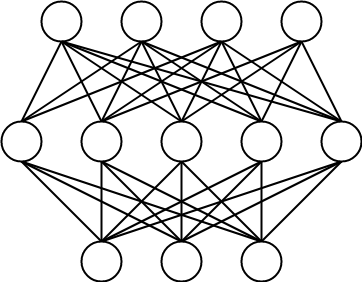
\includegraphics[scale=0.4]{fig/nn-blank.png}
			\caption{A schematic representation of a deep neural network.}
			\label{fig:nn-blank}
		\end{figure}
		\par One big advantage to using a neural network is the ability of the neural network to output multiple values. Instead of the neural network taking state-action pairs and output scalar values, they can instead take states as input and produce vectors of $Q$ values corresponding to the quality of each action in that state. This is a much more efficient approach. We call this network the \kword{$Q$-network} (DQN - deep $Q$-network for short). See figure \ref{fig:q-network-state-to-many-actions} for a schematic.
		\begin{figure}[ht]
			\centering
			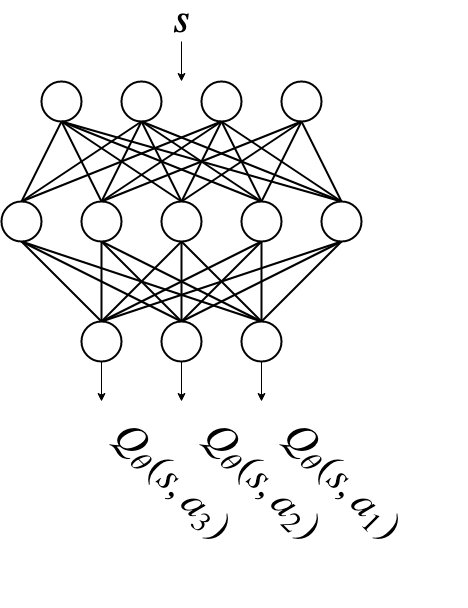
\includegraphics[scale=0.4]{fig/q-network-state-to-many-actions.png}
			\caption{A $Q$-network. The state is a 4-dimensional vector and there are 3 discrete actions available. The network takes a state $s$ as a parameter and for each action $a$ predicts the quality $Q(s,a;\theta)$ of that action.}
			\label{fig:q-network-state-to-many-actions}
		\end{figure}
		\par Neural networks need to be differentiable so that we can use the optimization technique of \kword{gradient descent} to train it. Typically a neural network is specified abstractly as a set of parameters $\theta$ that determine the output of the network given the input. We define a loss $L$ for the network that we want to minimize. Gradient descent works by taking the gradient of $L$ with respect to $\theta$ and taking a small step in the direction opposite the gradient (`down' the gradient, i.e., gradient descent). This is the basic formulation; several modern extensions of gradient descent exist that improve training of neural networks, the details of which we will not cover in this thesis.
		\par Consider the $Q$-learning update rule (\ref{eqn:q_update_rule}). When $Q_\pi(s_t, a_t)$ is exactly equal to the TD target, there is no update. Noticing this, we might consider the loss of our neural network to be 0 when the value for $Q(s_t, a_t)$ is equal to $r_t + \gamma \max_{a_{t+1}} Q(s_{t+1}, a_{t+1})$. This is exactly the framework of a regression problem. We can then define the loss to be the squared error between the two:
		\begin{equation}
			\label{eqn:q_loss_no_target_network}
			L(\theta) = \mathbb{E}_{a \sim \pi}[(y_i - Q(s, a; \theta))^2]
		\end{equation}
		where the TD target is $y_i$:
		\begin{equation}
			\label{eqn:y_i_no_target_network}
			y_i = \mathbb{E}_{a' \sim \pi} \big[ R_t + \gamma \max_{a'}Q(s', a'; \theta) \vert S_t = s, A_t = a \big]
		\end{equation}
		Note that here instead of writing $Q_\pi(s_t, a_t)$ we now write $Q(s_t, a_t; \theta)$. This is because our $Q$ value is now no longer driven by the policy of the agent; the policy is defined to be the greedy policy and the output of the $Q$ function is determined by the network parameters $\theta$ (as well as $s_t$ and $a_t$).

		\par Training the neural network would consist of the following sequence of events:
		\begin{enumerate}
			\item The agent in state $s_t$ calculates $Q(s_t, a_t; \theta)$ using network parameters $\theta$ for each possible $a_t$. Using the greedy policy, it selects the action $a_t$ that maximizes $Q(s_t, a_t; \theta)$.
			\item As a result of choosing this action, the state transitions to state $s_{t+1}$. The agent recieves a reward $r_t$ as a result.
			\item The agent is now in state $s_{t+1}$ calculates $Q(s_{t+1}, a_{t+1}; \theta)$ using network parameters $\theta$ for each possible $a_{t+1}$. The maximal value of $Q(s_{t+1}, a_{t+1}; \theta)$ is chosen.
			\item The network is trained to minimize the loss, with $Q(s_t, a_t; \theta)$ being the prediction of the network, and with $y_i$ being the reward for transitioning and the discounted maximal $Q$ value for state $s_{t+1}$ determined in step $4$ (i.e., $r_t + \gamma \max_{a_{t+1}}Q(s_{t+1}, a_{t+1}; \theta))$.
		\end{enumerate}
		See figure \ref{fig:state-transition-q-learning-loss} for a diagrammatic representation.

		\par To perform any variation of gradient descent requires defining the gradient of the loss function. In this case, we can just apply the chain rule to (\ref{eqn:y_i_no_target_network}). If we treat the TD target $y_i$ as a constant (which is appropriate), we get a rather simple expression for the gradient:
		\begin{equation}
			\label{eqn:q-learning-gradient-no-target}
			\nabla_\theta L(\theta) = \mathbb{E}_{a \sim \pi} \big[ 2(y_i - Q(s,a;\theta)) \nabla_\theta Q(s,a;\theta) \big]
		\end{equation}
		and to update the the network parameters, we simply use \kword{stochastic gradient descent}:
		\begin{equation}
			\label{eqn:SGD}
				\theta \gets \theta + \frac{1}{2} \alpha \nabla_\theta L(\theta)
		\end{equation}
		where $\alpha$ is the learning rate.

		\begin{figure}[ht]
			\centering
			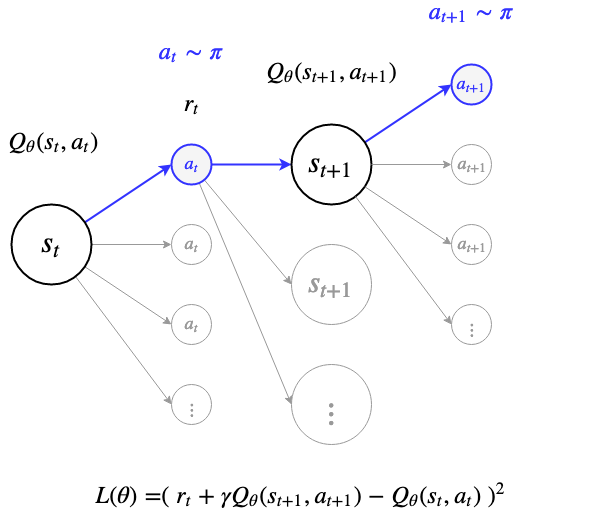
\includegraphics[scale=0.5]{fig/state-transition-q-learning-loss.png}
			\caption{A diagram showing how $Q$-learning gathers data for training.}
			\label{fig:state-transition-q-learning-loss}
		\end{figure}
		\subsection{Target Networks}
		\par One may have realized that this network $\theta$ is trying to predict it own output. This kind of learning is unstable, meaning performance can quickly deteriorate (to even worse than random \cite{worse_than_random}). One reason for this is that the neural network is differentiable. When we modify the parameters $\theta$ while training the network, we actually change the predictions for similar states to that which we just trained on. Research has shown that training can be stabilized by using two networks: $\theta_i$ and $\theta_{i-1}$. Instead of one set of parameters, we have two (i.e., we have two neural networks). We call the second network ($\theta_{i-1}$) the \kword{target network}, and it uses the parameters from the $Q$-network that synchronize with the current $Q$-network every $n_\theta$ timesteps.
		\par We define two policies:
		\begin{enumerate}
			\item $\mu$: The \kword{behaviour policy} that uses the $Q$-network ($Q(s,a;\theta_i)$) and is updated every time step.
			\item $\pi$: The \kword{target policy} that uses the target network ($Q(s',a';\theta_{i-1})$) and is updated to match $\mu$ (i.e., $\theta_{i-1}$ is updated to match $\theta_i$) every $n_\theta$ timesteps.
		\end{enumerate}
		The fact that the target network has fixed parameters for $n_\theta$ timesteps and predicts similarly to the $Q$-network stabilizes the learning.
		\par As a result, we get a new formulation of (\ref{eqn:q_loss_no_target_network}):
		\begin{equation}
				\label{eqn:q_loss_target_network}
				L_i(\theta_i) = \mathbb{E}_{a \sim \mu} \big[ (y_i - Q(s,a;\theta_i))^2 \big]
		\end{equation}
		where the TD target is $y_i$:
		\begin{equation}
			\label{eqn:y_i_target_network}
			y_i = \mathbb{E}_{a' \sim \pi} R_t + \gamma \max_{a'}Q(s', a'; \theta_{i-1}) \vert S_t = s, A_t = a]
		\end{equation}
		See figure \ref{fig:state-transition-q-learning-loss-target-networks} for a diagrammatic representation.
		\begin{figure}[ht]
			\centering
			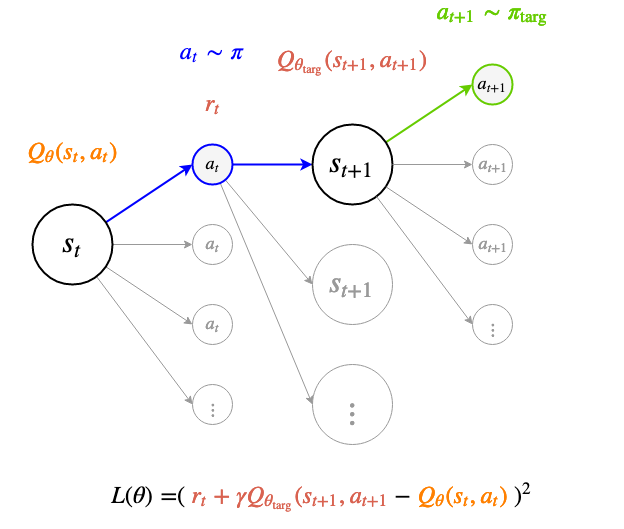
\includegraphics[scale=0.5]{fig/state-transition-q-learning-loss-target-networks.png}
			\caption{A diagram showing how $Q$-learning gathers data for training using the target network and behaviour network.}
			\label{fig:state-transition-q-learning-loss-target-networks}
		\end{figure}
		\subsection{Exploration-Exploitation}
		\par One major problem in RL is determining the optimal balance between \kword{exploration} and \kword{exploitation}. Exploitation refers to an agents tendency to choose actions that it thinks are best for it at any given time. This is the case with our greedy behaviour policy $\mu$. This comes at the cost of potentially not exploring new states that the agent has yet to visit. For the neural network to well approximate the $Q$ function, it needs to have exposure to as much of $\mc{S}$ as possible.
		\par One strategy is to select a constant $0 \leq \epsilon \leq 1$. We use $\epsilon$ to choose an action either randomly or according to $\mu$ by comparing a random number $p \sim \mc{U}(0,1)$ to $\epsilon$; if $p < \epsilon$ we choose a random action. Otherwise, we choose an action according to $\mu$.
		\par There are various strategies one can use for $\epsilon$-greedy policies. One example is to choose some initial value $\epsilon_i$ and some final value $\epsilon_f$, and a number of iterations $n_\epsilon$ over which $\epsilon_i$ decays into $\epsilon_f$. Another strategy is to choose $\epsilon$ empirically:
		$$\epsilon = \frac{1}{\sqrt{T+1}}$$
		where $T$ is the number of iterations (state transitions) in the episode.

		\subsection{Experience Replay}
		\par When we update out $Q$-network, we do it after every SARSA transition. Recall that we are using gradient descent to train the network parameters $\theta_i$. One problem with this is that we get a biased estimate for the gradient. A better estimate would involve taking the mean gradient estimate over many pairs of $Q(s,a)$ and TD targets. Furthermore, by training the network only on the most recent SARSA transition, we are making the network better at predicting the most recent TD target. This can actually undo some of the progress made training the network on earlier transitions. This problem is known as \kword{catastrophic forgetting}.
		\par We can solve the above problems by including an \kword{experience replay buffer} $\mc{D}$ that stores transitions
		$$\langle s_t, a_t, r_t, s_{t+1} \rangle$$
		Note that we do not need to store $a_{t+1}$ since our network will choose $a_{t+1}$ based on $\pi$ anyways.
		\par We then train the network by taking batches of transitions from $\mc{D}$. For each transition, we use the $Q$-network to predict $Q(s_t,a_t;\theta_i)$ and to consequently choose an action $a_t \sim \mu$, and we use the target network to predict $Q(s_{t+1},a_{t+1}; \theta_{i-1})$ and to consequently choose an action $a_{t+1} \sim \pi$. Over all transitions in the batch, we calculate the gradient of the loss $L_i(\theta_i)$ of the $Q$-network. We take the average of these gradients and update the network parameters.
		\subsection{Double $Q$-Learning}
		\par A common theme you may have noticed is that many developments in \kword{deep reinforcement learning} (using neural networks in RL) add new features to existing techniques. Above, we showed the addition of a target network, using an $\epsilon$-greedy action selection strategy, and using a memory replay buffer. Double $Q$-learning is another addition that builds on these.
		\par In the target network formulation of deep $Q$-learning, we use the target network to compute $Q(s_{t+1}, a_{t+1}; \theta_{i-1})$. We use $\pi$ to greedily choose an action $a_{t+1}$ as a result of this calculation. Thus, computing the quality of an action and choosing an action is tightly coupled. In double $Q$-learning, we decouple these.
		\par We choose an action $a_{t+1}$ based on the current behaviour policy $\mu$ (that is, we calculate $Q(s_{t+1},a_{t+1}; \theta_i)$ and select greedily from the results). We then use this $a_{t+1}$ to calculate $y_i$ (that is, we use $a_{t+1}$ to calculate $Q(s_{t+1}, a_{t+1}; \theta_{i-1})$). As a result, we can rewrite our TD target $y_i$:
		\begin{equation}
			\label{eqn:y_i_double}
			y_i = \mathbb{E}_{a' \sim \mu} \big[ r + \gamma Q(s', \arg \max_{a'} Q(s', a'; \theta_i); \theta_{i-1}) \big]
		\end{equation}
		See figure \ref{fig:state-transition-q-learning-loss-double} for a diagrammatic representation.
		\begin{figure}[ht]
			\centering
			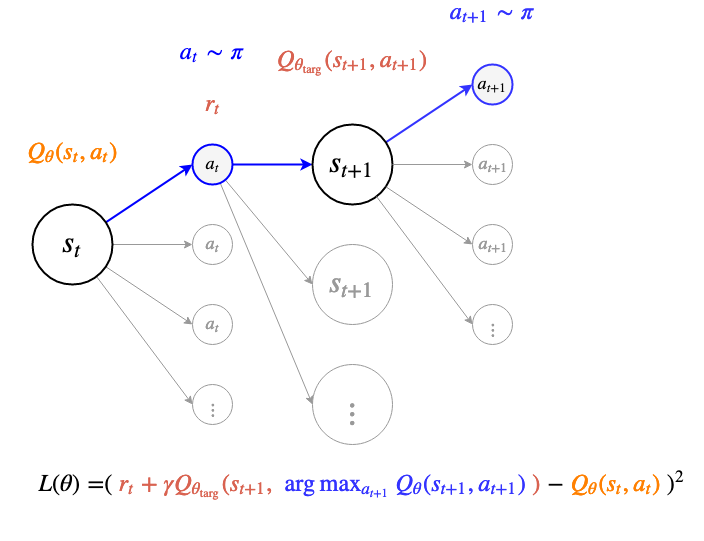
\includegraphics[scale=0.5]{fig/state-transition-q-learning-loss-double.png}
			\caption{A diagram showing how $Q$-learning gathers data for training using the double $Q$-learning.}
			\label{fig:state-transition-q-learning-loss-double}
		\end{figure}
		% \subsection{Duelling $Q$-Learning}
		% \par Above we have described the value of a state $V_\pi(s)$ and also the quality of taking a certain action $Q_\pi(s,a)$ (or in the case of DQNs, $Q(s, a; \theta)$). We can decompose the quality of a state-action pair $(s,a)$ into the base value of a state $s$ (how good it is to be in state $s$ in general) combined with some \kword{advantage} $A(s,a)$ of taking a certain action $a$ in state $s$ (how much better it is to take an action $a$ versus other actions).
		% \begin{align}
		% 	\label{eqn:advantage}
		% 	\begin{split}
		% 		Q_\pi(s,a) &= V_\pi(s) + A(s,a) \\
		% 		A(s,a) &= Q_\pi(s,a) - V_\pi(s)
		% 	\end{split}
		% \end{align}
		% Recall that $V_\pi(s)$ is the expected cumulative discounted reward starting in state $s$ and following the policy $\pi$, whereas $Q_\pi(s,a)$ is the expected cumulative discounted reward starting in state $s$ and taking action $a$, then following the policy $\pi$. In $V$, the policy provides the action; in $Q$, we do. Then the advantage $A$ essentially measure how much better (or worse) it is to take an action $a$ versus following the policy $\pi$ given a state $s$.
		% \par Overall, the advantage $A$ typically has a lower variance than the quality $Q$. Consider the calculation of the gradient (\ref{eqn:q-learning-gradient-no-target}) which is proportional to the magnitude of the quality; a high variance in the gradient means a poorer estimate of the true gradient and thus worse training. With this in mind, we might consider an architecture called a \kword{duelling $Q$-network} that shares most of its network parameters, but has two outputs: a single output for $V(s)$ and multiple outputs for $Q(s,a)$ which it uses to predict the advantage $A(s,a)$ for each action $a$ (see figure \ref{fig:duelling-q-network}).
		% \begin{figure}[ht]
		% 	\centering
		% 	\includegraphics[scale=0.5]{fig/duelling-q-network.png}
		% 	\caption{A schematic of a duelling $Q$-network. }
		% 	\label{fig:duelling-q-network}
		% \end{figure}
		\section{Policy Gradient}
		\par In $Q$-learning, we have a policy $\pi$ that is simply a greedy (or $\epsilon$-greedy) strategy. While this can be effective in problems with small action spaces, we may face problems with large (or continuous) action spaces. We can circumvent this by instead directly trying to model $\pi$. We can parametrize the policy using some parameters $\theta$ to produce a distribution over actions:
		\begin{equation}
			\label{eqn:policy-as-distribution}
			\pi_\theta(a, s) = \mathbb{P}\big[ A_t=a \vert S_t = s; \theta \big]
		\end{equation}
		\par Modelling the policy directly has an additional advantage over the greedy policy from $Q$-learning, which is that it can learn a \kword{stochastic policy}. We have the option of picking an action stochastically over the distribution $\pi$.
		\par Consider some objective function $J$ that we want to optimize using our policy (and consequently $J$ is a function of $\theta$). An obvious choice would be the expected rewards over all possible \kword{trajectories} $\tau$ (that is, sequences of states, actions, and rewards):
		\begin{equation}
			\label{eqn:j-expectation}
			J(\theta) = \mathbb{E}_{\pi_\theta} \big[ r(\tau) \big]
		\end{equation}
		where $r(\tau)$ represents the total reward over a trajectory $\tau$. Finding an optimal policy $\pi_\theta$ amounts to finding a set of parameters $\theta$ that maximizes $J$. One way to do this is to use a differentiable function approximator for $\pi$ such that we can perform \kword{stochastic gradient ascent}
		\begin{equation}
			\label{eqn:j-SGA}
			\theta \gets \theta + \alpha \nabla_\theta J(\theta)
		\end{equation}
		\subsection{The Policy Gradient Theorem}
		This simple formulation is rather decieving. We now have the rather difficult task of evaluating $\nabla_\theta J(\theta)$.
		\begin{align}
			\begin{split}
			\label{eqn:j-as-integral-over-tau}
			J(\theta) &= \mathbb{E}_{\pi_\theta} \big[ r(\tau) \big] \\
			&= \int \pi_\theta (\tau) r(\tau) d \tau
		\end{split}
		\end{align}
		So we express the expectation of the reward over all trajectories $\tau$ as expected to be followed using policy $\pi$. Here, $\pi_\theta (\tau)$ represents the probability of generating the trajectort $\tau$ using policy $\pi_\theta$. The gradient of $J$ is
		\begin{equation}
			\label{eqn:nabla-j-as-integral-over-tau}
			\nabla_\theta J(\theta) = \int \nabla_\theta \pi_\theta (\tau) r(\tau) d \tau \\
		\end{equation}
		We can use the following identity:
		\begin{align}
			\label{eqn:nabla_log_identity}
			\nabla_\theta \pi_\theta (\tau) &= \pi_\theta (\tau) \frac{\nabla_\theta \pi_\theta (\tau)}{\pi_\theta (\tau)} \\
			&= \pi_\theta (\tau) \nabla_\theta \log \pi_\theta (\tau)
	\end{align}
	and substitute it into (\ref{eqn:nabla-j-as-integral-over-tau}) to get
	\begin{align}
		\label{eqn:nabla-j-with-log}
		\nabla_\theta J(\theta) &= \int \pi_\theta (\tau) \nabla_\theta \log \pi_\theta (\tau) r(\tau) d \tau \\
		&= \mathbb{E}_{\pi_\theta} \big[ \nabla_\theta \log \pi_\theta (\tau) r(\tau)\big] \nonumber
	\end{align}
	We now need to consider the probability $\pi_\theta (\tau)$ of generating a trajectory $\tau$. Let us define $d$ to be the distribution of states, and let $s_0$ denote an initial state. Let the trajectory $\tau$ be over time steps $1, 2, \dots, T$.
	\begin{equation}
		\label{eqn:probability_of_generating_tau}
		\pi_\theta (\tau) = d(s_0) \prod_{t=1}^T \pi_\theta (a_t \vert s_t; \theta) \mc{P}_{s_t, a_t, s_{t+1}}
	\end{equation}
	We can read this as being the probability of being in an initial state AND the probability of choosing an action $a_t$ given the state $s_t$ and policy parameters $\theta$ AND the probability of transitioning to state $s_{t+1}$ given the current state and action. In (\ref{eqn:nabla-j-with-log}) we are taking the $\log$ of $\pi_\theta (\tau)$. Doing so to (\ref{eqn:probability_of_generating_tau}) yields:
	\begin{equation}
		\label{eqn:log_probablity_of_generating_tau}
		\log \pi_\theta (\tau) = \log d(s_0) + \sum_{t=1}^T \log \pi_\theta (a_t \vert s_t; \theta) + \log \mc{P}_{s_t, a_t, s_{t+1}}
	\end{equation}
	Finally, we take the gradient with respect to $\theta$:
	\begin{equation}
		\label{eqn:nabla_log_probablity_of_generating_tau}
		\nabla_\theta \log \pi_\theta (\tau) = \nabla_\theta \sum_{t=1}^T \log \pi_\theta (a_t \vert s_t; \theta)
	\end{equation}
	It turns out that since neither the distribution of states $d$ nor the dynamics of the MDP $\mc{P}$ have an impact on the gradient! Thus, we finally get an expression for the gradient $\nabla_\theta J(\theta)$:
	\begin{equation}
		\label{eqn:policy_gradient_theorem}
		\nabla_\theta J(\theta) = \mathbb{E}_{\pi_\theta} \bigg[ \nabla_\theta \sum_{t=1}^T \log \pi_\theta (a_t \vert s_t; \theta) r(\tau) \bigg]
	\end{equation}
	We call this \kword{the policy gradient theorem}. In fact, it is a slight variant of the policy gradient theorem where we use specific trajectories of actions rather than taking the expectation over all actions, but for implementation purposes it is sufficient \cite{sutton}.
	\subsection{REINFORCE}
	\par You may note that $r(\tau)$ above remains essentially untouched. In fact, since, past rewards don't influence future rewards, we may replace it with $G_t$ (i.e., the return from time point $t$ onwards). If we wish to take an expectation of this, we must sample trajectories. This requires knowing in advance the return $G_t$, which consequently requires the agent to finish an episode before updating parameters. This method of sampling complete trajectories and then making updates is called \kword{episodic Monte Carlo policy gradient control}. It is episodic because the agent finishes an episode before updating. It is Monte Carlo because it samples complete trajectories according to the policy before making updates. This gives a modified version of (\ref{eqn:policy_gradient_theorem}):
	\begin{equation}
		\label{eqn:policy_gradient_theorem_G_t}
		\nabla_\theta J(\theta) = \mathbb{E}_{\pi_\theta} \bigg[ \nabla_\theta \sum_{t=1}^T \log \pi_\theta (a_t \vert s_t; \theta) G_t \bigg]
	\end{equation}
	 By considering this gradient, we get the REINFORCE algorithm:
	\begin{equation}
		\label{eqn:REINFORCE}
		\theta_{t+1} \gets \theta_{t} + \alpha \nabla_{\theta_t} \log \pi_{\theta_t}(a_t \vert s_t; \theta_t) G_t
	\end{equation}
	At this point, it may be useful to undo the identity (\ref{eqn:nabla_log_identity}) and intuitively deconstruct why the REINFORCE update rules makes sense:
	$$\theta_{t+1} \gets \theta_{t} + \alpha  \frac{\nabla_{\theta_t} \pi_{\theta_t}(a_t \vert s_t; \theta_t)}{\pi_{\theta_t}(a_t \vert s_t; \theta_t)} G_t$$
	The gradient vector on the top of the fraction points in the direction (in parameter space) that most increases the probability of taking action $a_t$ in state $s_t$. Using this alone could lead to a feedback loop where the agent continually makes itself more likely to choose this action over and over, so as a result, we divide it by the probability of taking that action. Finally, we scale it by the return to encourage behaviours that maximize the return.
	\subsection{Actor-Critic Models (AC)}
	\par The issue with the REINFORCE method is that it is a Monte Carlo method. First, it can be prohibitively slow to train, performing updates to the policy only after episode completion. Second, the Monte Carlo sampling approach can be extremely high variance (for example, maybe in one episode $G_t$ is 100 and in another it is $0$). Third, it requires training to be episodic (instead of ongoing). This motivates the development of the \kword{actor-critic} model.
	\par The actor-critic model combines the techniques of policy gradient and also $Q$-learning. Rather than completing entire episodes $G_t$ and then updating (as in REINFORCE), we could simply try to estimate the quality of a state-action pair $(s,a)$ and update the policy after each time step. This is exactly the goal of $Q$-learning. Let us use a function approximator (again, often a neural network) parametrized by some parameters $\phi$ to predict $Q_{\pi_\theta}(s,a)$ This gives us an approximation to the gradient of our objective function:
	\begin{equation}
		\label{eqn:j-approximation}
		\nabla_\theta J(\theta) \approx \mathbb{E}_{\pi_\theta} \big[ \nabla_\theta \log \pi_\theta(s,a; \theta) Q_{\pi_\theta}(s,a; \phi) \big]
	\end{equation}
	\par We now have two sets of parameters to optimize. We can optimize $\theta$ (the actor) using the policy gradient in (\ref{eqn:j-approximation}) and we can use deep $Q$-learning to optimize $\phi$.\footnote{The compatible function approximation theorem gives conditions under which the equality is exact. See \ref{deepmind} for details.}
	\subsection{Advantage Actor Critic (A2C)}
	\par Consider an environment where the rewards are not highly informative of the `goodness' of choosing certain actions over others (e.g., the rewards are $100,103,102,\dots$). Conceptually, this means that the quality of choosing an action $a$ in a state $s$ is mostly just the value of the state $V(s)$. The difference in expected return between choosing an action $a$ (as in the quality) versus just following the policy from state $s$ onwards (as in the value) is called the \kword{advantage} $A(s,a)$ of choosing action $a$ in state $s$:
	\begin{align}
		\label{eqn:advantage}
		Q_{\pi_\theta}(s,a) &= V_{\pi_\theta}(s) + A_{\pi_\theta}(s,a) \\
		A_{\pi_\theta}(s,a) &= Q_{\pi_\theta}(s,a) - V_{\pi_\theta}(s) \nonumber
	\end{align}
	\par Clearly the advantage is a better estimate of the `goodness' of certain actions, and furthermore has lower variance. We just need to confirm that substituting the advantage in for the quality of normal actor-critic models does not change our expectation in (\ref{eqn:j-approximation}).

	\begin{align}
		\label{eqn:policy_gradient_theorem_with_baseline}
		\begin{split}
			\nabla_\theta J(\theta) &= \mathbb{E}_{\pi_\theta} \bigg[ \nabla_\theta \sum_{t=1}^T \log \pi_\theta (a_t \vert s_t; \theta) \big( Q_{\pi_\theta}(s,a) - V_{\pi_\theta}(s) \big) \bigg] \\
			\mathbb{E}_{\pi_\theta} \bigg[ \nabla_\theta \sum_{t=1}^T \log \pi_\theta (a_t \vert s_t; \theta) V_{\pi_\theta}(s) \bigg] &= \int
		\end{split}
	\end{align}

	\subsection{PPO}
	\section{Intrinsic Motivation}
	\subsection{Sparse Rewards}
	\subsection{ICM}
	\subsection{Go-Explore}
	\subsection{Episodic Curiosity through Reachability}
	\section{Sparse Distributed Memory}




	% \bibliographystyle{IEEEtran}
	% \bibliography{references}

\end{document}
